\documentclass[a4paper, 12pt]{report}

% Чтобы работала кириллица
\usepackage[T2A]{fontenc}
\usepackage[utf8]{inputenc}

% Делаем человеческие отступы (экономим бумагу)
\usepackage[left=1.3cm,right=1.3cm,top=2cm,bottom=2cm]{geometry}

% Чтобы можно было вставлять кириллицу в формулы
\usepackage{amsmath}

% Вставляем картинки
\usepackage{graphicx}
\usepackage{epstopdf}

% Для ссылок во всемирную сеть
\usepackage{nohyperref}  % This makes hyperref commands do nothing without errors
\usepackage{url}  % This makes \url work


% Меняем подпись рисунков и таблиц на русский
\renewcommand{\figurename}{Рис.}
\renewcommand{\tablename}{Табл.}

% Title Page
\title{Отчет о проделанной работе за следующую неделю}
\author{Зелинский Виктор}
\date{22 апреля 2024}


\begin{document}
	\maketitle
	\newpage
	\section{Проделанная работа}
	Я пересчитал графики для границ применимости с единичными параметрами (\figurename \ref{fig:euler_ones})
	\begin{figure}[h]
		\includegraphics[width=0.9\linewidth]{big_plot500(ones).png}
		\caption{Графики энергии для различных значений кинетической, потенциальной и суммарной энергией}
		\label{fig:euler_ones}
	\end{figure}

	Также реализовал периодические граничные условия и снова исследовал границы применимости (\figurename \ref{fig:euler_periodical})
	
	\begin{figure}[h]
		\includegraphics[width=0.9\linewidth]{big_plot100(periodical).png}
		\caption{Графики энергии для различных значений кинетической, потенциальной и суммарной энергией}
		\label{fig:euler_periodical}
	\end{figure}
	
	Сменил схему с Эйлера на Верле, исследовал границы применимости(правда пока на маленьком количестве шагов и параметров) (\figurename \ref{fig:verlet})

	\begin{figure}[h]
		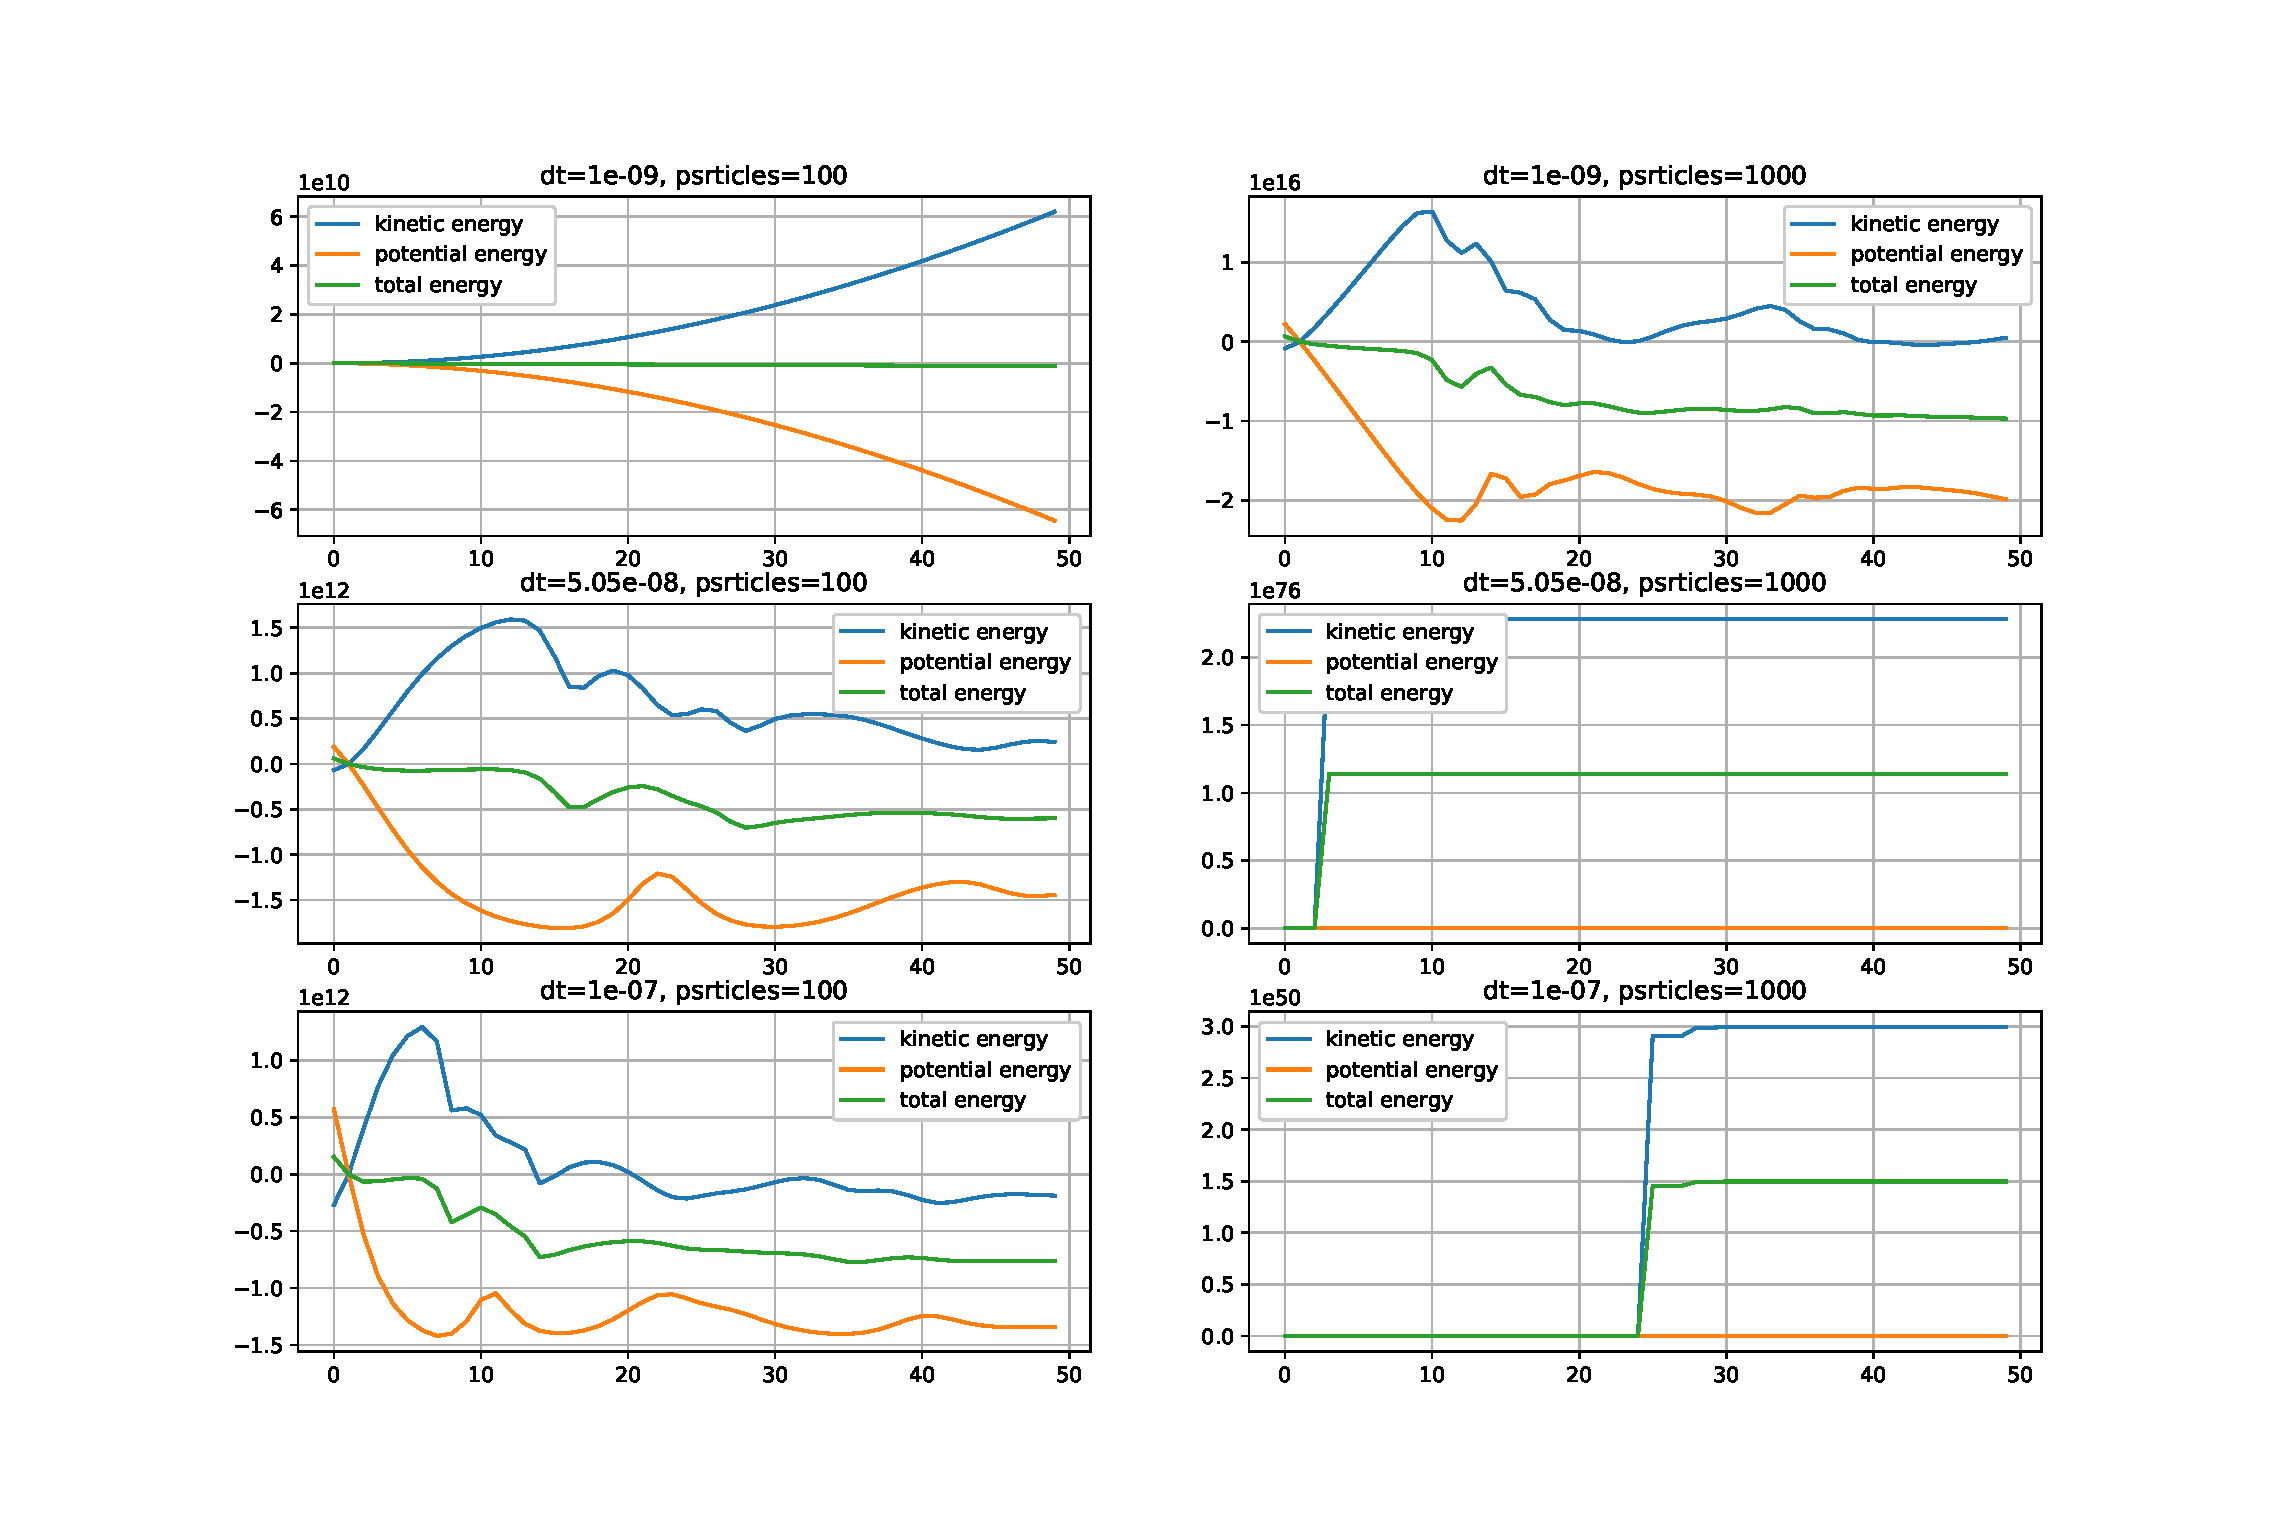
\includegraphics[width=0.9\linewidth]{big_plot50(periodical).eps}
		\caption{Графики энергии для различных значений кинетической, потенциальной и суммарной энергией}
		\label{fig:verlet}
	\end{figure}

	\section{Выводы}
	\begin{enumerate}
		\item С периодическими граничными условиями флуктуации энергии больше, но разлет системы происходит при больших значениях параметров (более устойчиво).
		\item Несмотря на меньшее количество графиков для схемы Верле, уже можно сделать вывод, что система более стабильна. 
	\end{enumerate}
\end{document}          
